\documentclass[12pt, a4paper]{article}
\setlength{\textheight}{24cm}
\setlength{\textwidth}{16cm}
\setlength{\topmargin}{0cm}
\setlength{\evensidemargin}{0cm}
\setlength{\oddsidemargin}{0cm}
\usepackage[affil-it]{authblk}
\usepackage{graphics}
\usepackage{graphicx}
\usepackage{caption}
\usepackage{float}
\usepackage[british]{babel}
\usepackage{hyperref}
\usepackage{subcaption}
\date{}
\begin{document}
\title{Comparison of several frameworks for general-purpose programming and the  computation of FFTs on GPUs}
\author{Philippe Gambron \thanks{\texttt{philippe.gambron{@}stfc.ac.uk}}, Sue Thorne \thanks{\texttt{sue.thorne{@}stfc.ac.uk}}}
\affil{Science and Technology Facilities Council, Hartree Centre, Rutherford Appleton Laboratory, Harwell Campus, Harwell Oxford, OX11 0QZ, United Kingdom}
\maketitle
\begin{abstract}
We compare the performance of several frameworks that can be used, in C, for general-purpose programming on a graphical processing unit (GPU) or to compute Fast Fourier Transforms (FFTs).  
\end{abstract}
\section{Introduction}
For a bit more than a decade, the use of GPU has become increasingly widespread. They are indeed capable of significantly increasing the performance of a single workstation or compute node. While there are some overheads associated to the t data transfers between the memory and the GPU and the launch of the kernel and some constraints on the types of algorithms can be efficiently programmed, one can obtain tremendous performance gains on suitable problems.\\

In this report, we will compare the performance of several of these frameworks that we measured for a simple general-purpose programming example and for computing FFTs on the GPU by using the libraries provided by these frameworks. 

\section{Overview of the chosen libraries}
We consider the following frameworks for GPU programming: CUDA \cite{cuda}, OpenCL \cite{opencl}, OpenMP \cite{openmp}\footnote{From version 4.0, OpenMP offers GPU programming} and Kokkos \cite{kokkos}. The first three of these frameworks provide as well FFT libraries. Respectively, they are: cuFFT \cite{cufft}, clFFT \cite{clfft} and AccFFT \cite{accfft} (Table \ref{ffttable}). They can perform complex transforms, real-to-half-complex ones (and conversely) as well as, in the case of FFTW, real-to-real transforms when the signal is odd or even. The half-complex output consists in half as many complex values as there were points in the signal, taking advantage of the hermiticity of the Fourier transform of a real function.\\ 
\begin{table}[H]
\captionsetup{width=1\textwidth}
\begin{tabular}{|p{2.5cm}||p{2.5cm}|p{1cm}|p{3cm}|p{3cm}|p{2cm}|p{2cm}|}
\hline
& Type & Dim. & Radices & Licence \\
\hline
\hline
AccFFT & R$\to$H,\ \ \  C$\to$C& 3& & GPL v2\\
\hline
clFFT  &  R$\to$H,\ \ \  C$\to$C,\ \ \ \  H$\to$R& 1, 2, 3 & 2, 3, 5, 7 & Proprietary\\
\hline
cuFFT  &  R$\to$H,\ \ \  C$\to$C,\ \ \ \  H$\to$R & 1, 2, 3 & 2, 3, 5, 7 & GPL v3\\
\hline
\end{tabular}
\caption{Overview of the FFT libraries considered. R stands for real, C, for complex, and HC, for half-complex.}
\label{ffttable}
\end{table}
\section{Benchmark}
The benchmark \cite{code} consists in calculating the FFT of a series of volumes, in 1, 2 or 3 dimensions, of real or complex values. The purpose was to mimick a problem submitted to us by the CCP PET-MR collaboration \cite{ccppetmr}, within the Software Outlook initiative \cite{softwareoutlook}, who needed to take the transform of series of square complex images. This example is depicted in Fig. \ref{benchmark}. For our more general test, the 2-dimensional slices could be replaced by a line or a rectangular cuboid. We used 32 images, which was a typical value used by that collaboration, for the tests that were representative of their requirement. For the other runs, we always processed a single image.\\

\begin{figure}[H]
\captionsetup{width=0.6\textwidth}
\centering
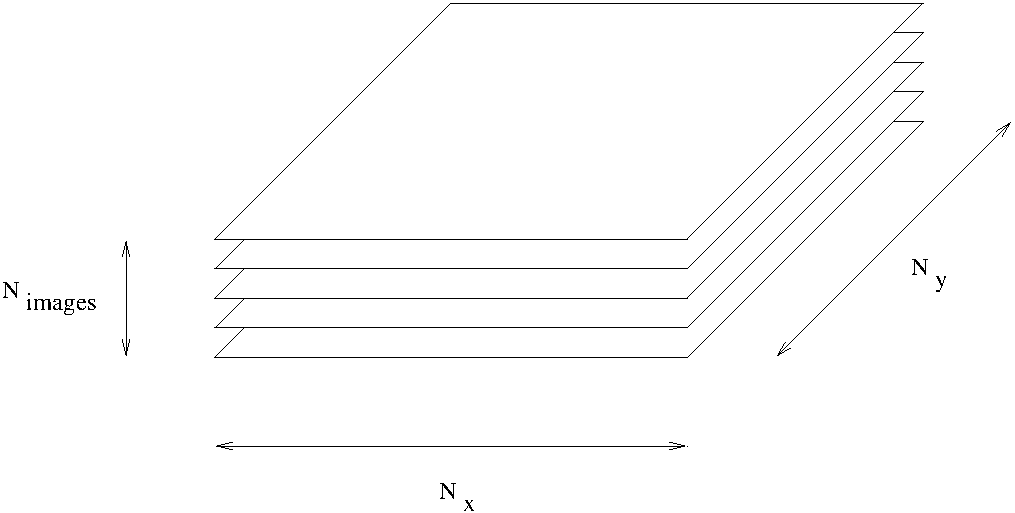
\includegraphics[height=5cm]{benchmark.pdf}
\caption{The benchmark consists in taking the FFT of several images. Each of them is made of real or complex values and can be a simple line, a rectangle or a cuboid.}
\label{benchmark}
\end{figure}

We used a number of points varying from $\sim 10^3$ to $\sim 10^7$. The domains had sides of equal lengths (square or cubic) or were flattened (rectangle or cuboid). These dimensions could be powers of 2, products of powers of small integers (2, 3, 5 and 7) or prime numbers. The values appearing in the graphs are the execution times averaged over 10 runs.

\section{Setup}

The measurements were carried out on a system featuring an Intel Xeon W-2133 CPU (6 cores, 3.6 GHz), a NVIDIA Quadro GV100 GPU and 12 GB of RAM. We used the following GPU programming frameworks: CUDA (version 10.0.130), OpenCL (version 1.2.7) and  

\section{Product}

\begin{figure}[H]
\captionsetup{width=0.8\linewidth}
\centering
\begin{subfigure}{.5\textwidth}
\centering
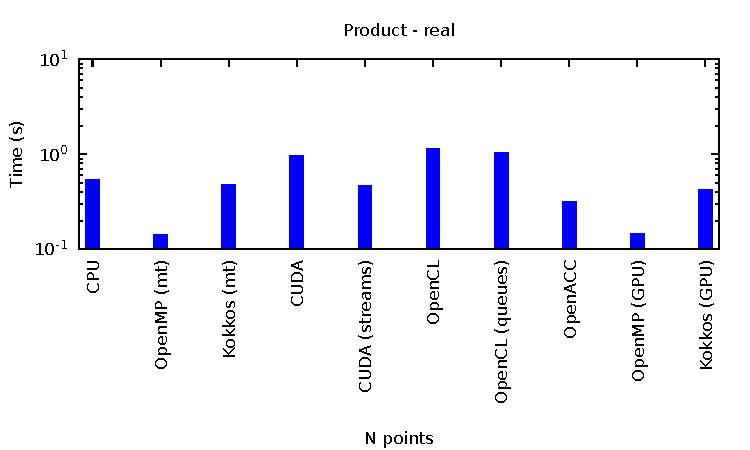
\includegraphics[width=.9\linewidth]{graphs/product-r.pdf}
\caption{Real numbers}
\label{PRODR}
\end{subfigure}%
\begin{subfigure}{.5\textwidth}
\centering
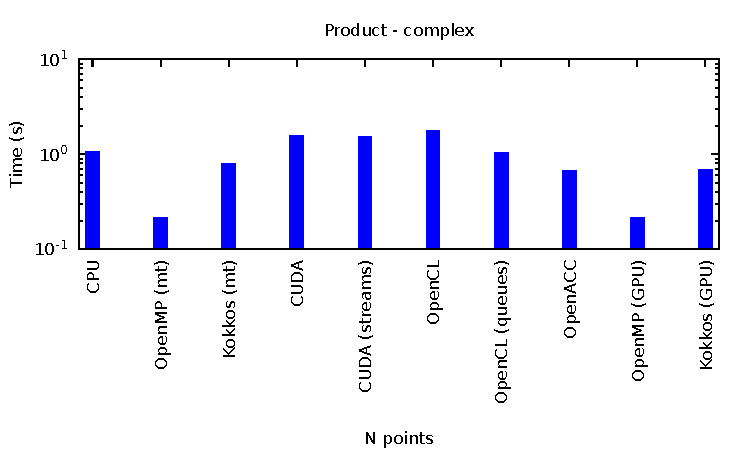
\includegraphics[width=.9\linewidth]{graphs/product-c.pdf}
\caption{Complex numbers}
\label{PRODC}
\end{subfigure}
\caption{Execution time for the product of a large number of $2^{24}$ real and complex points using several frameworks.}
\label{1DFFTW}
\end{figure}



\section{Fast Fourier Transform}
\subsection{Effect of the problem size - One dimension}





\begin{figure}[H]
\captionsetup{width=0.8\linewidth}
\centering
\begin{subfigure}{.5\textwidth}
\centering
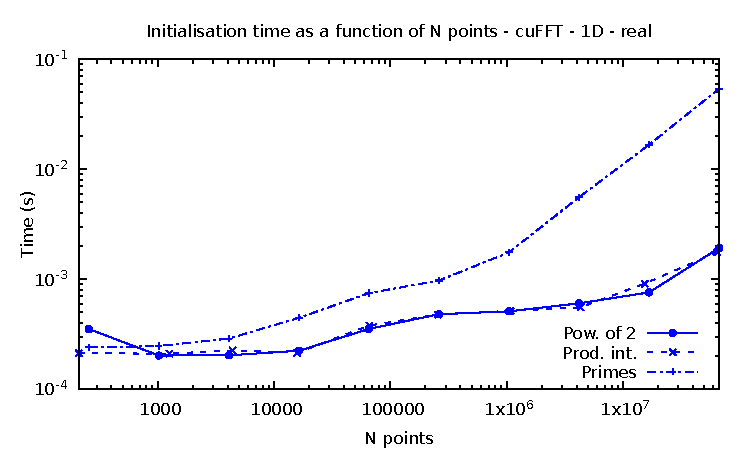
\includegraphics[width=.9\linewidth]{graphs/fft-cuda-1d-pow2-r-init.pdf}
\caption{Intialisation (real)}
\label{FFTCUDA1DRI}
\end{subfigure}%
\begin{subfigure}{.5\textwidth}
\centering
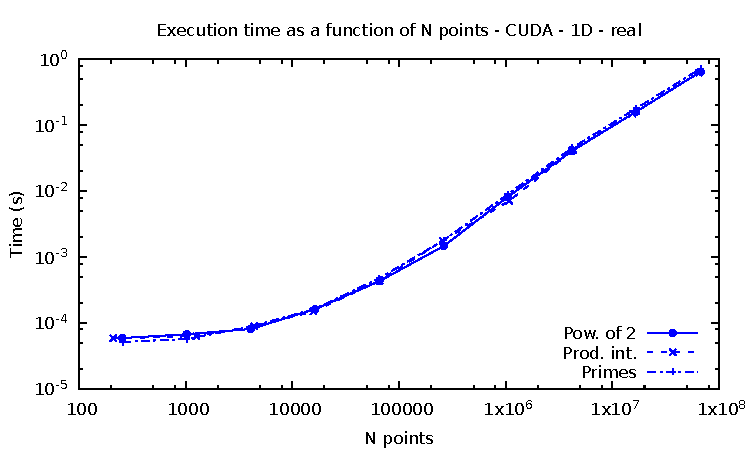
\includegraphics[width=.9\linewidth]{graphs/fft-cuda-1d-pow2-r-exec.pdf}
\caption{Execution (real)}
\label{FFTCUDA1DRE}
\end{subfigure}\\
\begin{subfigure}{.5\textwidth}
\centering
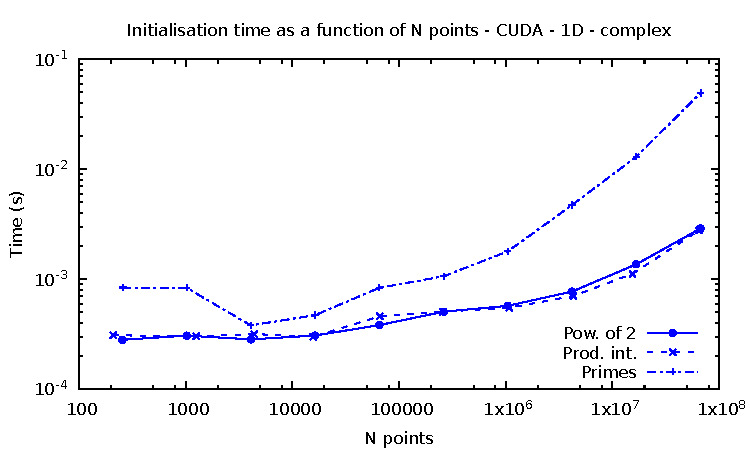
\includegraphics[width=.9\linewidth]{graphs/fft-cuda-1d-pow2-c-init.pdf}
\caption{Intialisation (complex)}
\label{FFTCUDA1DCI}
\end{subfigure}%
\begin{subfigure}{.5\textwidth}
\centering
\includegraphics[width=.9\linewidth]{graphs/fft-cuda-1d-pow2c-exec.pdf}
\caption{Execution (complex)}
\label{FFTCUDA1DCE}
\end{subfigure}
\caption{Initialisation and execution times as a function of the number of points\\(1 dimension)}
\label{FFTCUDA1D}
\end{figure}


\begin{figure}[H]
\captionsetup{width=0.8\linewidth}
\centering
\begin{subfigure}{.5\textwidth}
\centering
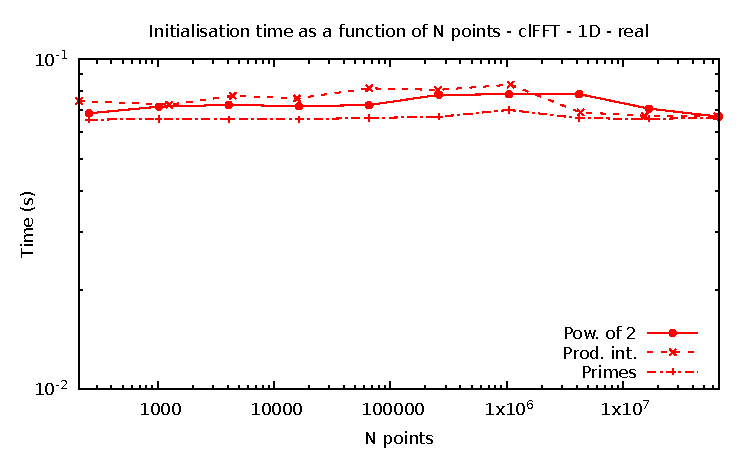
\includegraphics[width=.9\linewidth]{graphs/fft-opencl-1d-pow2-r-init.pdf}
\caption{Intialisation (real)}
\label{FFTCL1DRI}
\end{subfigure}%
\begin{subfigure}{.5\textwidth}
\centering
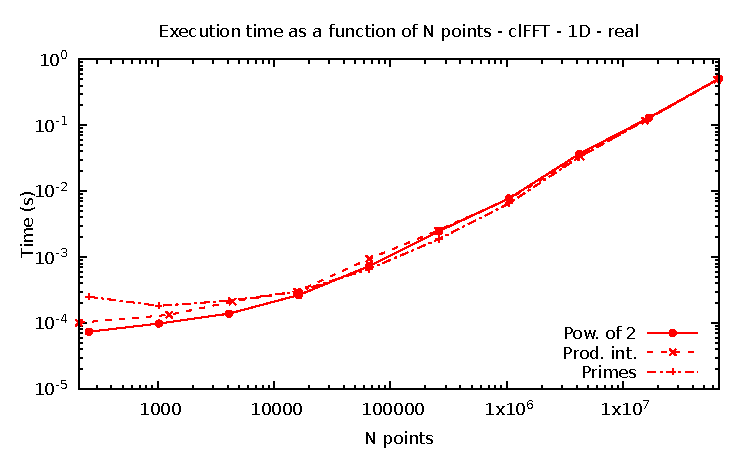
\includegraphics[width=.9\linewidth]{graphs/fft-opencl-1d-pow2-r-exec.pdf}
\caption{Execution (real)}
\label{FFTCL1DRE}
\end{subfigure}\\
\begin{subfigure}{.5\textwidth}
\centering
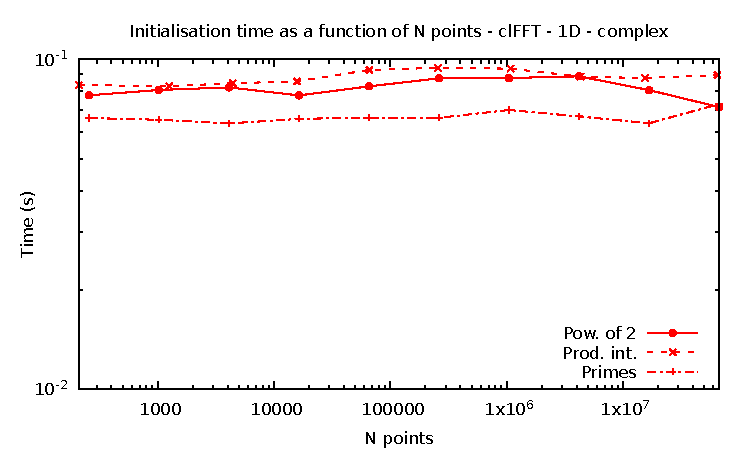
\includegraphics[width=.9\linewidth]{graphs/fft-opencl-1d-pow2-c-init.pdf}
\caption{Intialisation (complex)}
\label{FFTCL1DCI}
\end{subfigure}%
\begin{subfigure}{.5\textwidth}
\centering
\includegraphics[width=.9\linewidth]{graphs/fft-opencl-1d-pow2c-exec.pdf}
\caption{Execution (complex)}
\label{FFTCL1DCE}
\end{subfigure}
\caption{Initialisation and execution times as a function of the number of points\\(1 dimension)}
\label{FFTCL1D}
\end{figure}



\begin{figure}[H]
\captionsetup{width=0.8\linewidth}
\centering
\begin{subfigure}{.5\textwidth}
\centering
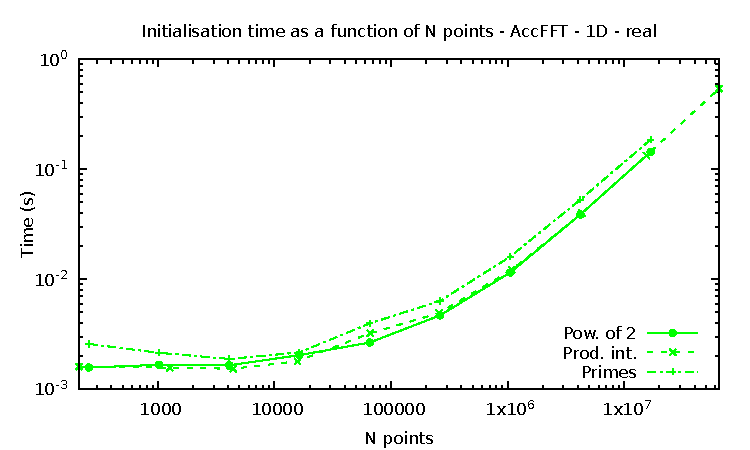
\includegraphics[width=.9\linewidth]{graphs/fft-openacc-1d-pow2-r-init.pdf}
\caption{Intialisation (real)}
\label{FFTACC1DRI}
\end{subfigure}%
\begin{subfigure}{.5\textwidth}
\centering
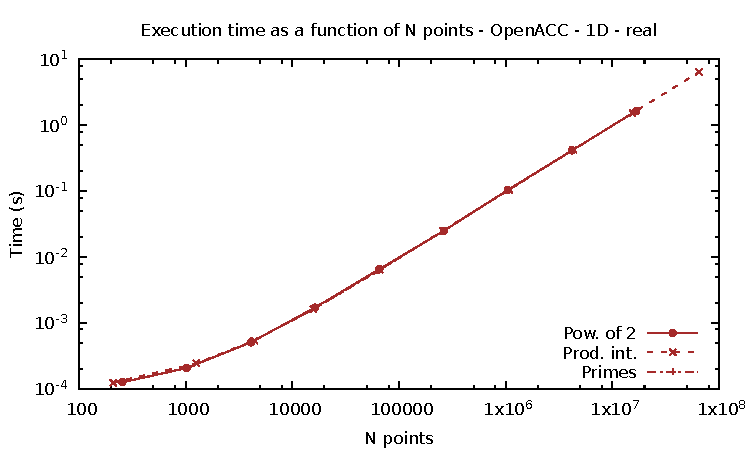
\includegraphics[width=.9\linewidth]{graphs/fft-openacc-1d-pow2-r-exec.pdf}
\caption{Execution (real)}
\label{FFTACC1DRE}
\end{subfigure}\\
\begin{subfigure}{.5\textwidth}
\centering
%\includegraphics[width=.9\linewidth]{}
\caption{Intialisation (complex)}
\label{FFTACC1DCI}
\end{subfigure}%
\begin{subfigure}{.5\textwidth}
\centering
\includegraphics[width=.9\linewidth]{graphs/fft-openacc-1d-pow2c-exec.pdf}
\caption{Execution (complex)}
\label{FFTACC1DCE}
\end{subfigure}
\caption{Initialisation and execution times as a function of the number of points\\(1 dimension)}
\label{FFTCL1D}
\end{figure}



\begin{figure}[H]
\captionsetup{width=0.8\linewidth}
\centering
\begin{subfigure}{.5\textwidth}
\centering
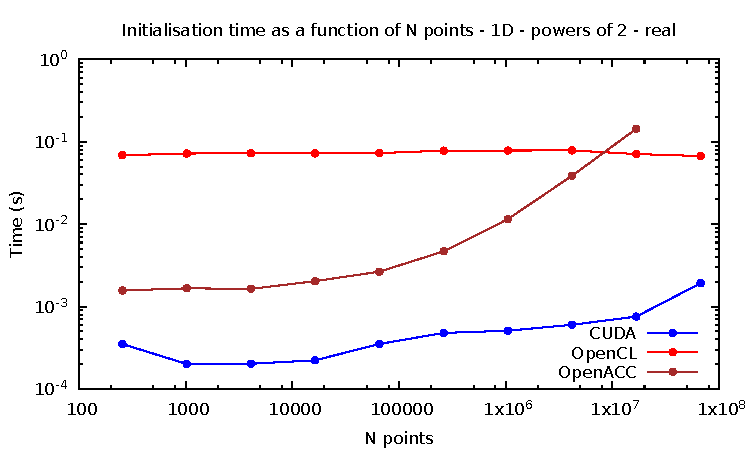
\includegraphics[width=.9\linewidth]{graphs/fft-1d-pow2-r-init.pdf}
\caption{Intialisation (real)}
\label{FFTPOW21DRI}
\end{subfigure}%
\begin{subfigure}{.5\textwidth}
\centering
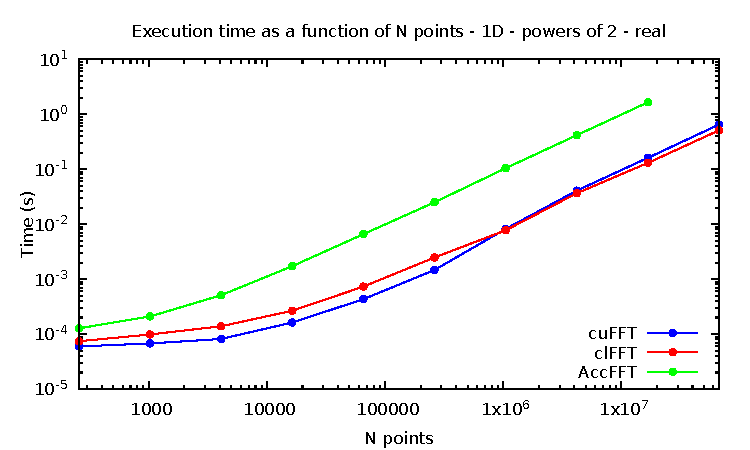
\includegraphics[width=.9\linewidth]{graphs/fft-1d-pow2-r-exec.pdf}
\caption{Execution (real)}
\label{FFTPOW21DRE}
\end{subfigure}\\
\begin{subfigure}{.5\textwidth}
\centering
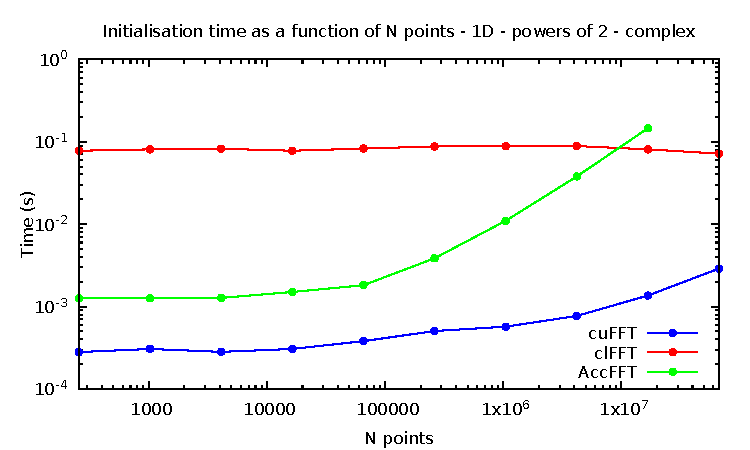
\includegraphics[width=.9\linewidth]{graphs/fft-1d-pow2-c-init.pdf}
\caption{Intialisation (complex)}
\label{FFTPOW21DCI}
\end{subfigure}%
\begin{subfigure}{.5\textwidth}
\centering
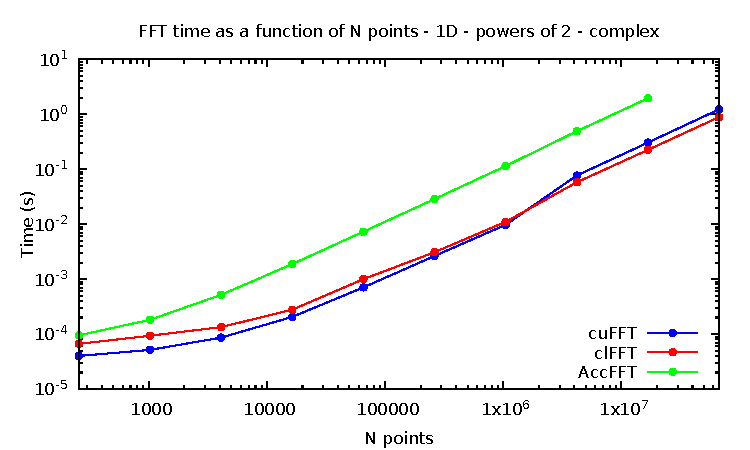
\includegraphics[width=.9\linewidth]{graphs/fft-1d-pow2-c-exec.pdf}
\caption{Execution (complex)}
\label{FFTPOW21DCE}
\end{subfigure}
\caption{Initialisation and execution times as a function of the number of points\\(1 dimension)}
\label{FFTPOW21D}
\end{figure}


\begin{figure}[H]
\captionsetup{width=0.8\linewidth}
\centering
\begin{subfigure}{.5\textwidth}
\centering
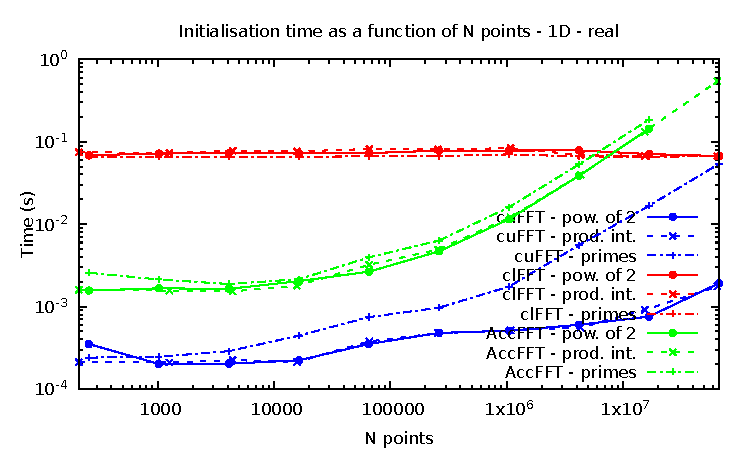
\includegraphics[width=.9\linewidth]{graphs/fft-1d-r-init.pdf}}
\caption{Intialisation (real)}
\label{FFT1DRI}
\end{subfigure}%
\begin{subfigure}{.5\textwidth}
\centering
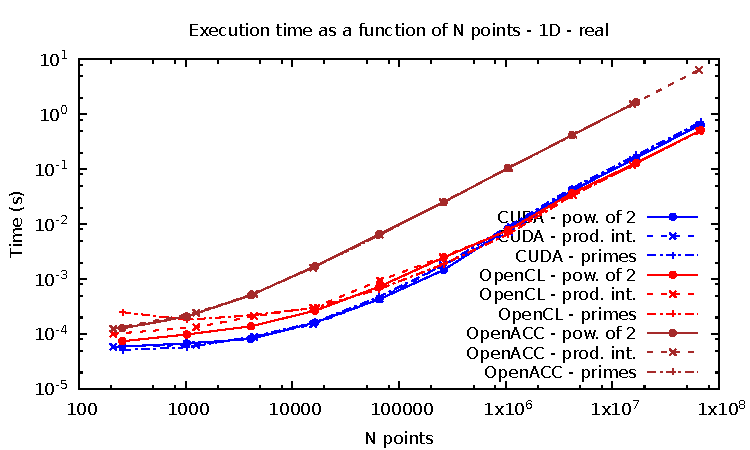
\includegraphics[width=.9\linewidth]{graphs/fft-1d-r-exec.pdf}
\caption{Execution (real)}
\label{FFT1DRE}
\end{subfigure}\\
\begin{subfigure}{.5\textwidth}
\centering
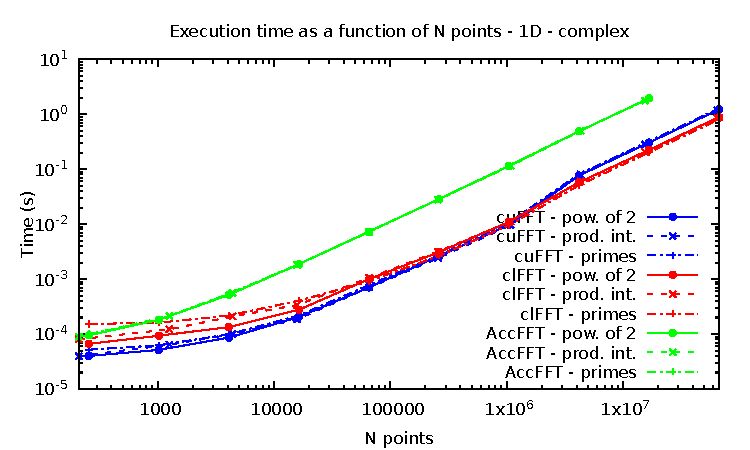
\includegraphics[width=.9\linewidth]{graphs/fft-1d-c-exec.pdf}
\caption{Intialisation (complex)}
\label{FFT1DCI}
\end{subfigure}%
\begin{subfigure}{.5\textwidth}
\centering
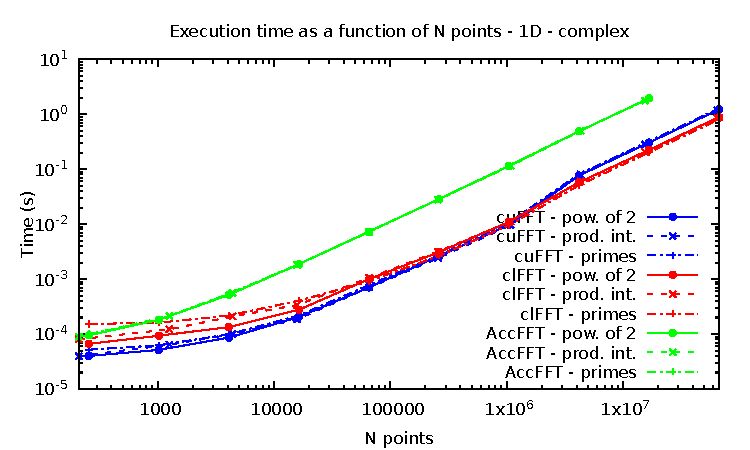
\includegraphics[width=.9\linewidth]{graphs/fft-1d-c-exec.pdf}
\caption{Execution (complex)}
\label{FFT1DCE}
\end{subfigure}
\caption{Initialisation and execution times as a function of the number of points\\(1 dimension)}
\label{FFT1D}
\end{figure}

\subsection{Effect of the problem size - Two dimensions}

\begin{figure}[H]
\captionsetup{width=0.8\linewidth}
\centering
\begin{subfigure}{.5\textwidth}
\centering
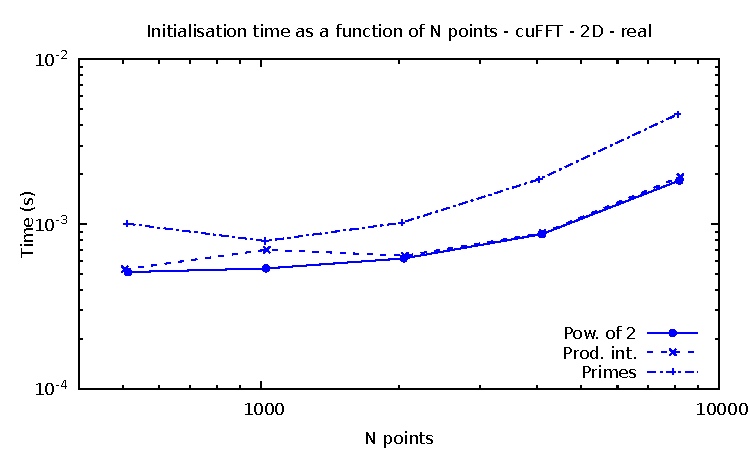
\includegraphics[width=.9\linewidth]{graphs/fft-cuda-2d-pow2-r-init.pdf}
\caption{Intialisation (real)}
\label{FFTCUDA1DRI}
\end{subfigure}%
\begin{subfigure}{.5\textwidth}
\centering
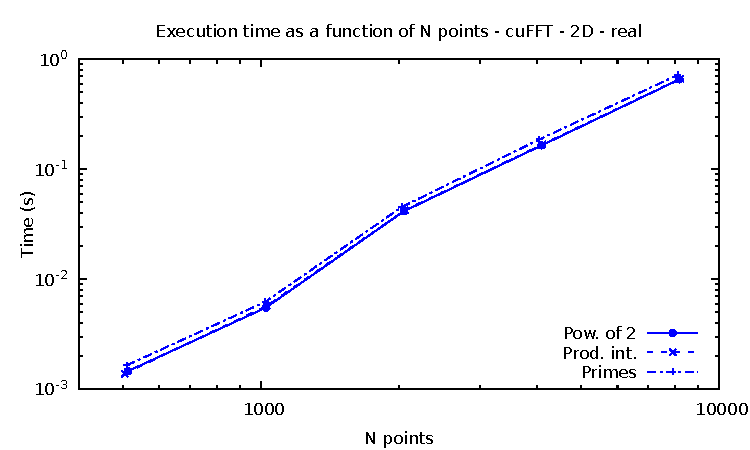
\includegraphics[width=.9\linewidth]{graphs/fft-cuda-2d-pow2-r-exec.pdf}
\caption{Execution (real)}
\label{FFTCUDA1DRE}
\end{subfigure}\\
\begin{subfigure}{.5\textwidth}
\centering
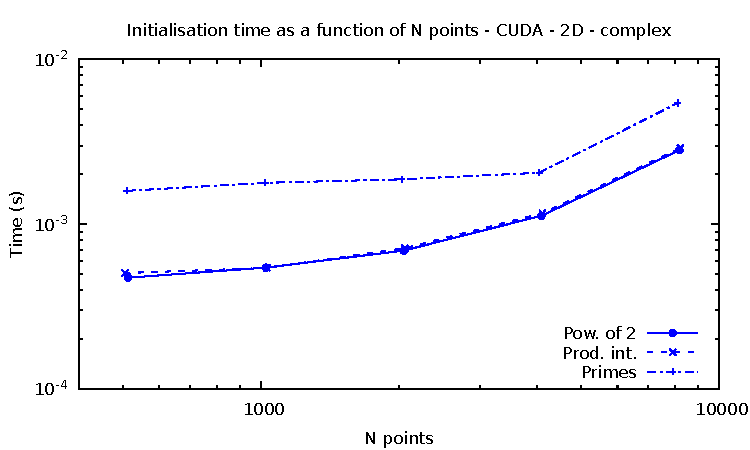
\includegraphics[width=.9\linewidth]{graphs/fft-cuda-2d-pow2-c-init.pdf}
\caption{Intialisation (complex)}
\label{FFTCUDA1DCI}
\end{subfigure}%
\begin{subfigure}{.5\textwidth}
\centering
\includegraphics[width=.9\linewidth]{graphs/fft-cuda-2d-pow2c-exec.pdf}
\caption{Execution (complex)}
\label{FFTCUDA1DCE}
\end{subfigure}
\caption{Initialisation and execution times as a function of the number of points\\(1 dimension)}
\label{FFTCUDA1D}
\end{figure}

\begin{figure}[H]
\captionsetup{width=0.8\linewidth}
\centering
\begin{subfigure}{.5\textwidth}
\centering
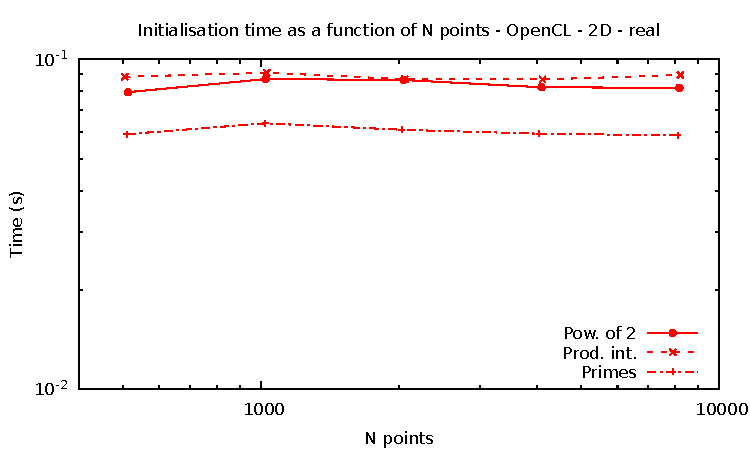
\includegraphics[width=.9\linewidth]{graphs/fft-opencl-2d-pow2-r-init.pdf}
\caption{Intialisation (real)}
\label{FFTCL1DRI}
\end{subfigure}%
\begin{subfigure}{.5\textwidth}
\centering
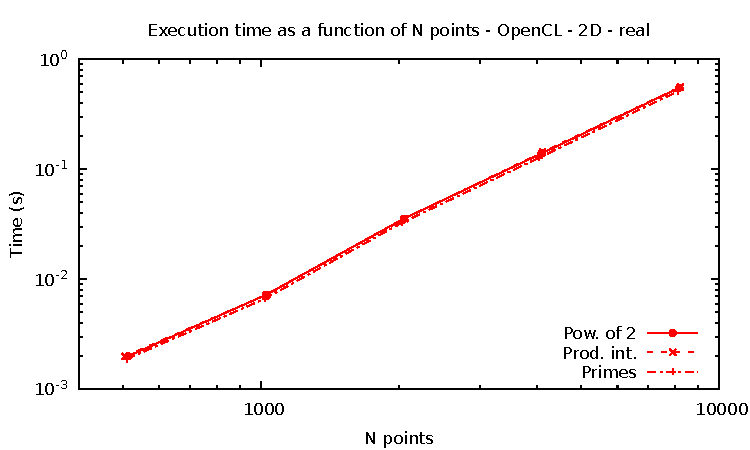
\includegraphics[width=.9\linewidth]{graphs/fft-opencl-2d-pow2-r-exec.pdf}
\caption{Execution (real)}
\label{FFTCL1DRE}
\end{subfigure}\\
\begin{subfigure}{.5\textwidth}
\centering
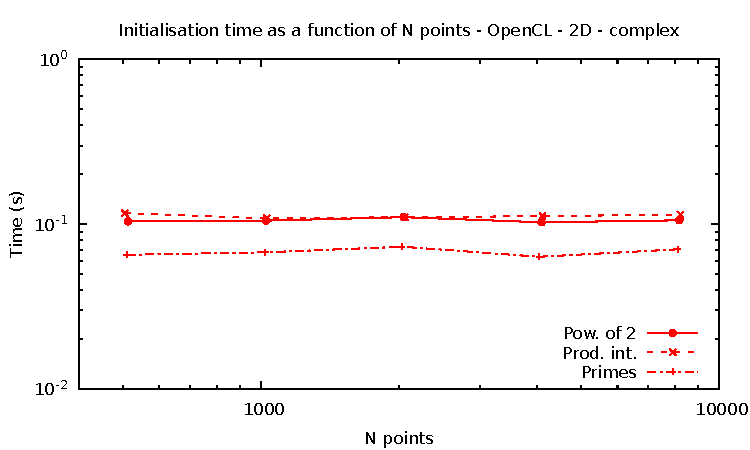
\includegraphics[width=.9\linewidth]{graphs/fft-opencl-2d-pow2-c-init.pdf}
\caption{Intialisation (complex)}
\label{FFTCL1DCI}
\end{subfigure}%
\begin{subfigure}{.5\textwidth}
\centering
\includegraphics[width=.9\linewidth]{graphs/fft-opencl-2d-pow2c-exec.pdf}
\caption{Execution (complex)}
\label{FFTCL1DCE}
\end{subfigure}
\caption{Initialisation and execution times as a function of the number of points\\(1 dimension)}
\label{FFTCL1D}
\end{figure}


\begin{figure}[H]
\captionsetup{width=0.8\linewidth}
\centering
\begin{subfigure}{.5\textwidth}
\centering
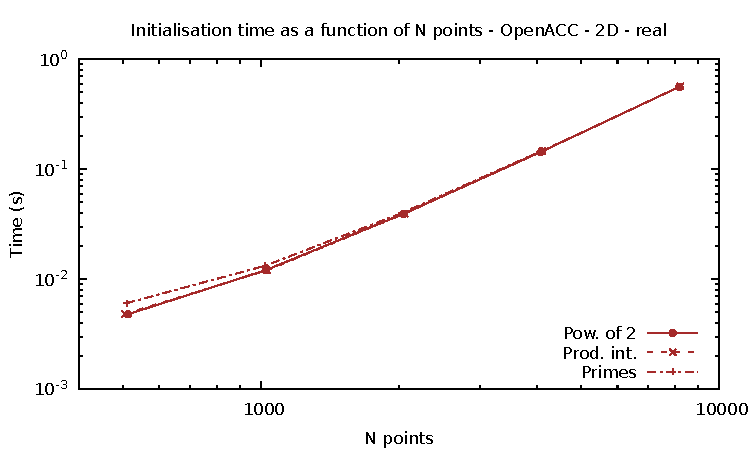
\includegraphics[width=.9\linewidth]{graphs/fft-openacc-2d-pow2-r-init.pdf}
\caption{Intialisation (real)}
\label{FFTACC1DRI}
\end{subfigure}%
\begin{subfigure}{.5\textwidth}
\centering
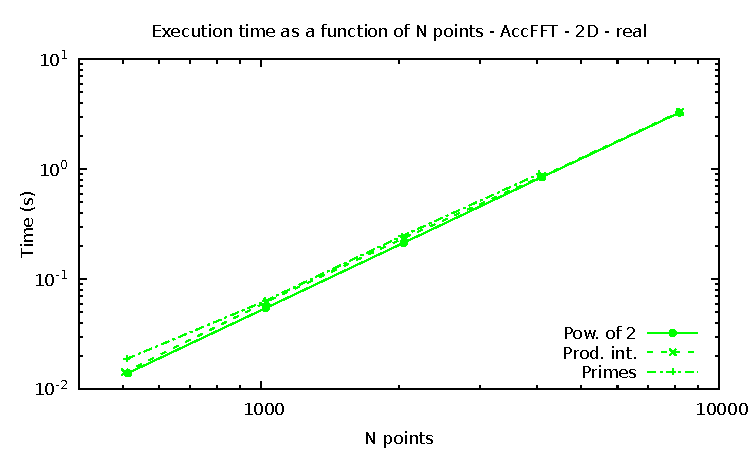
\includegraphics[width=.9\linewidth]{graphs/fft-openacc-2d-pow2-r-exec.pdf}
\caption{Execution (real)}
\label{FFTACC1DRE}
\end{subfigure}\\
\begin{subfigure}{.5\textwidth}
\centering
%\includegraphics[width=.9\linewidth]{}
\caption{Intialisation (complex)}
\label{FFTACC1DCI}
\end{subfigure}%
\begin{subfigure}{.5\textwidth}
\centering
\includegraphics[width=.9\linewidth]{graphs/fft-openacc-2d-pow2c-exec.pdf}
\caption{Execution (complex)}
\label{FFTACC1DCE}
\end{subfigure}
\caption{Initialisation and execution times as a function of the number of points\\(1 dimension)}
\label{FFTCL1D}
\end{figure}

\begin{figure}[H]
\captionsetup{width=0.8\linewidth}
\centering
\begin{subfigure}{.5\textwidth}
\centering
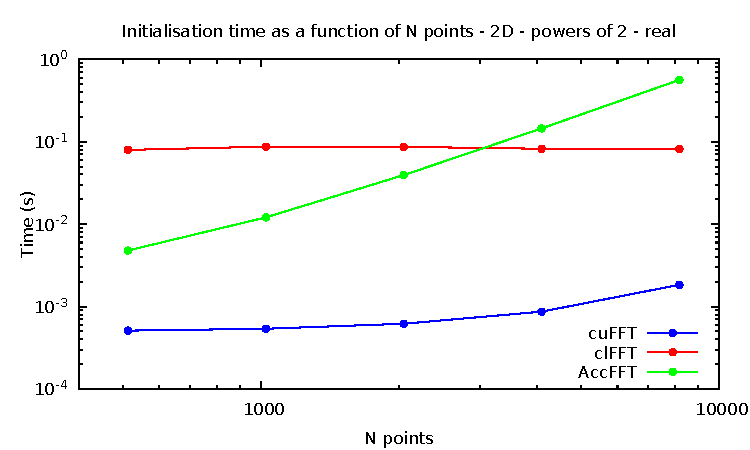
\includegraphics[width=.9\linewidth]{graphs/fft-2d-pow2-r-init.pdf}
\caption{Intialisation (real)}
\label{FFTPOW21DRI}
\end{subfigure}%
\begin{subfigure}{.5\textwidth}
\centering
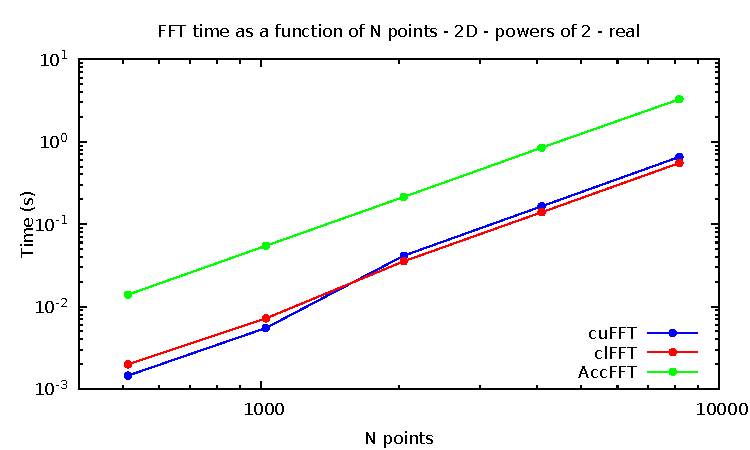
\includegraphics[width=.9\linewidth]{graphs/fft-2d-pow2-r-exec.pdf}
\caption{Execution (real)}
\label{FFTPOW21DRE}
\end{subfigure}\\
\begin{subfigure}{.5\textwidth}
\centering
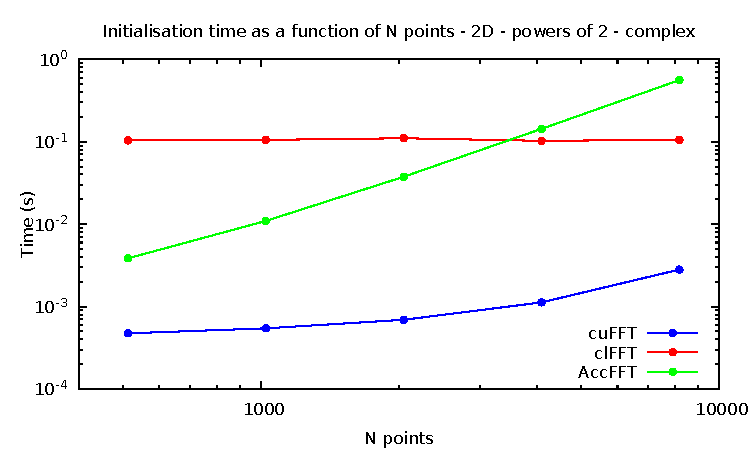
\includegraphics[width=.9\linewidth]{graphs/fft-2d-pow2-c-init.pdf}
\caption{Intialisation (complex)}
\label{FFTPOW21DCI}
\end{subfigure}%
\begin{subfigure}{.5\textwidth}
\centering
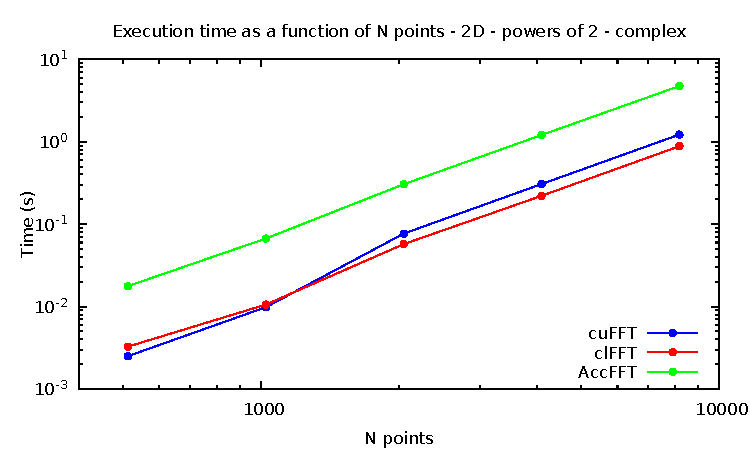
\includegraphics[width=.9\linewidth]{graphs/fft-2d-pow2-c-exec.pdf}
\caption{Execution (complex)}
\label{FFTPOW21DCE}
\end{subfigure}
\caption{Initialisation and execution times as a function of the number of points\\(1 dimension)}
\label{FFTPOW21D}
\end{figure}

\begin{figure}[H]
\captionsetup{width=0.8\linewidth}
\centering
\begin{subfigure}{.5\textwidth}
\centering
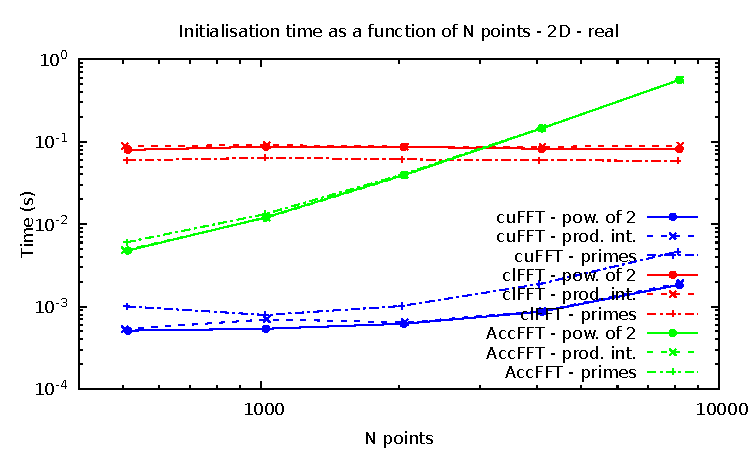
\includegraphics[width=.9\linewidth]{fft-2d-r-init.pdf}}
\caption{Intialisation (real)}
\label{FFT1DRI}
\end{subfigure}%
\begin{subfigure}{.5\textwidth}
\centering
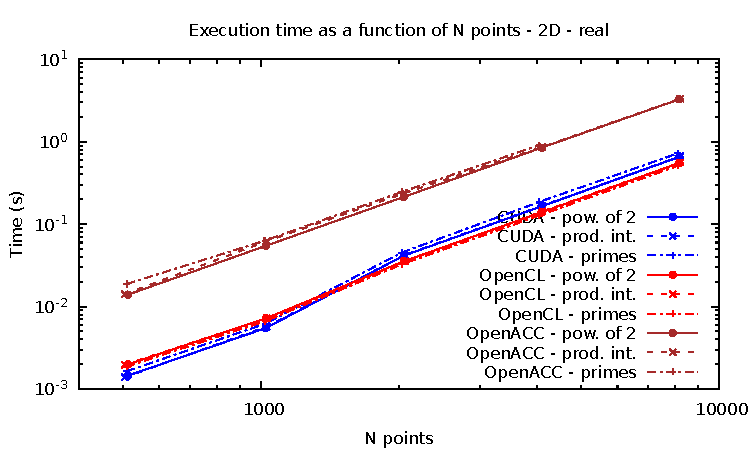
\includegraphics[width=.9\linewidth]{graphs/fft-2d-r-exec.pdf}
\caption{Execution (real)}
\label{FFT1DRE}
\end{subfigure}\\
\begin{subfigure}{.5\textwidth}
\centering
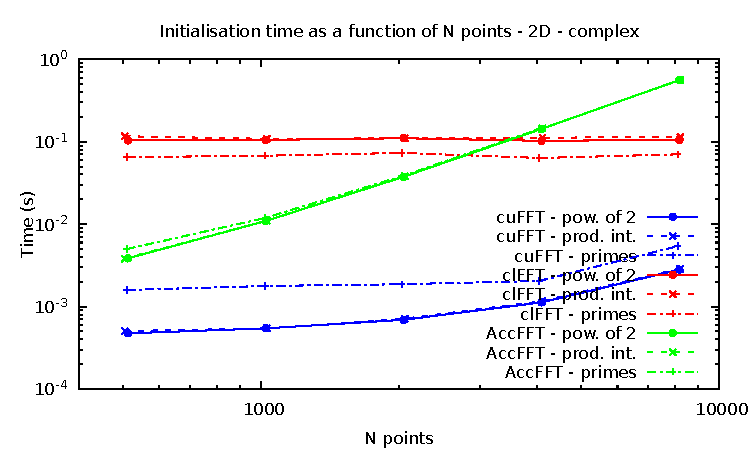
\includegraphics[width=.9\linewidth]{graphs/fft-2d-c-init.pdf}
\caption{Intialisation (complex)}
\label{FFT1DCI}
\end{subfigure}%
\begin{subfigure}{.5\textwidth}
\centering
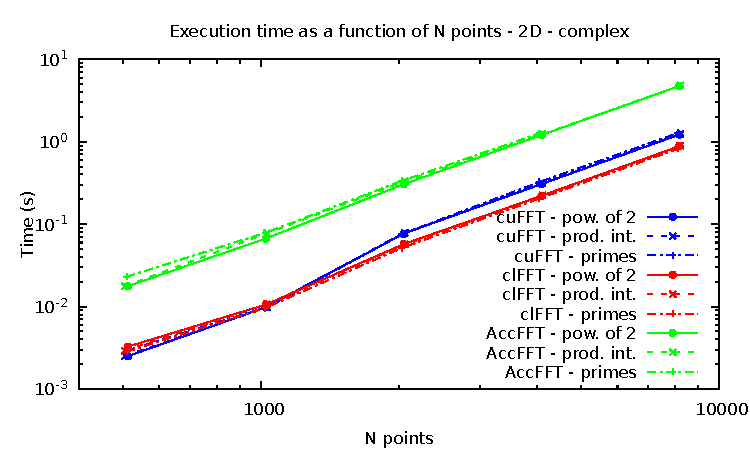
\includegraphics[width=.9\linewidth]{graphs/fft-2d-c-exec.pdf}
\caption{Execution (complex)}
\label{FFT1DCE}
\end{subfigure}
\caption{Initialisation and execution times as a function of the number of points\\(1 dimension)}
\label{FFT1D}
\end{figure}







\subsection{Effect of the problem size - Three dimensions}

\begin{figure}[H]
\captionsetup{width=0.8\linewidth}
\centering
\begin{subfigure}{.5\textwidth}
\centering
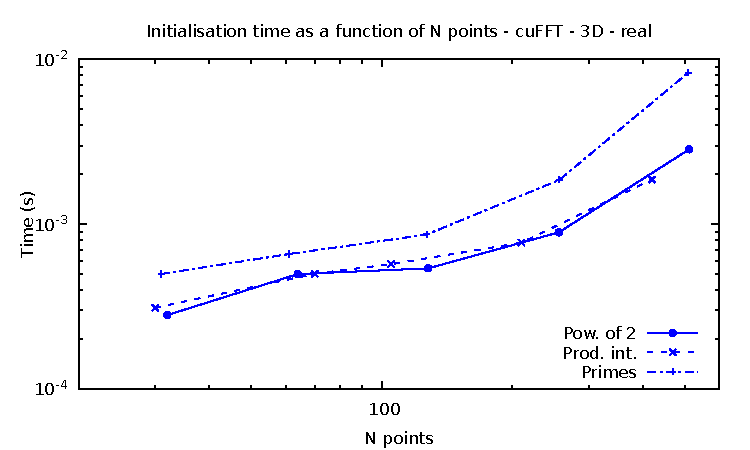
\includegraphics[width=.9\linewidth]{graphs/fft-cuda-3d-pow2-r-init.pdf}
\caption{Intialisation (real)}
\label{FFTCUDA1DRI}
\end{subfigure}%
\begin{subfigure}{.5\textwidth}
\centering
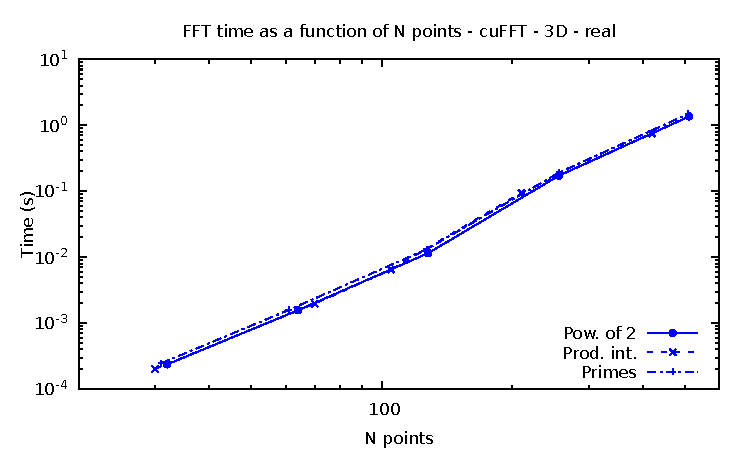
\includegraphics[width=.9\linewidth]{graphs/fft-cuda-3d-pow2-r-exec.pdf}
\caption{Execution (real)}
\label{FFTCUDA1DRE}
\end{subfigure}\\
\begin{subfigure}{.5\textwidth}
\centering
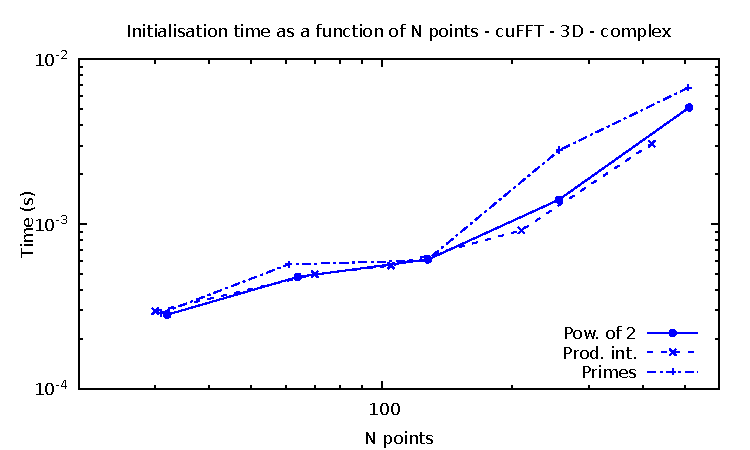
\includegraphics[width=.9\linewidth]{graphs/fft-cuda-3d-pow2-c-init.pdf}
\caption{Intialisation (complex)}
\label{FFTCUDA1DCI}
\end{subfigure}%
\begin{subfigure}{.5\textwidth}
\centering
\includegraphics[width=.9\linewidth]{graphs/fft-cuda-3d-pow2c-exec.pdf}
\caption{Execution (complex)}
\label{FFTCUDA1DCE}
\end{subfigure}
\caption{Initialisation and execution times as a function of the number of points\\(1 dimension)}
\label{FFTCUDA1D}
\end{figure}



\begin{figure}[H]
\captionsetup{width=0.8\linewidth}
\centering
\begin{subfigure}{.5\textwidth}
\centering
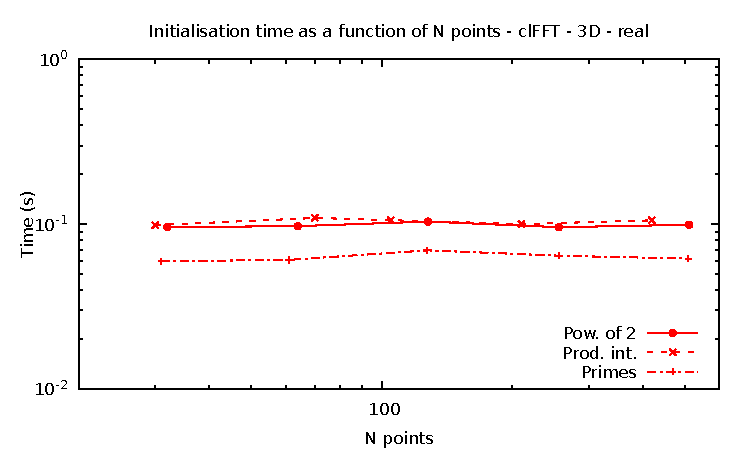
\includegraphics[width=.9\linewidth]{graphs/fft-opencl-3d-pow2-r-init.pdf}
\caption{Intialisation (real)}
\label{FFTCL1DRI}
\end{subfigure}%
\begin{subfigure}{.5\textwidth}
\centering
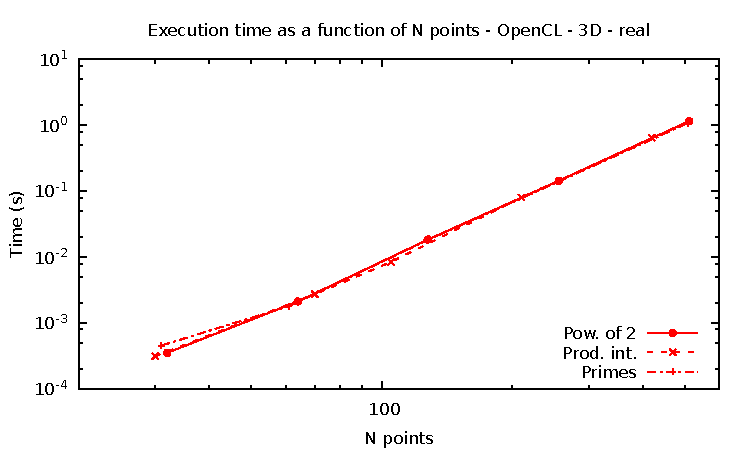
\includegraphics[width=.9\linewidth]{graphs/fft-opencl-3d-pow2-r-exec.pdf}
\caption{Execution (real)}
\label{FFTCL1DRE}
\end{subfigure}\\
\begin{subfigure}{.5\textwidth}
\centering
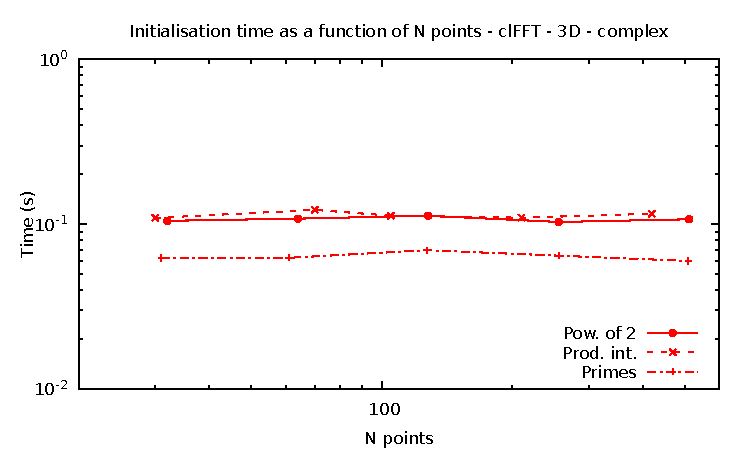
\includegraphics[width=.9\linewidth]{graphs/fft-opencl-3d-pow2-c-init.pdf}
\caption{Intialisation (complex)}
\label{FFTCL1DCI}
\end{subfigure}%
\begin{subfigure}{.5\textwidth}
\centering
\includegraphics[width=.9\linewidth]{graphs/fft-opencl-3d-pow2c-exec.pdf}
\caption{Execution (complex)}
\label{FFTCL1DCE}
\end{subfigure}
\caption{Initialisation and execution times as a function of the number of points\\(1 dimension)}
\label{FFTCL1D}
\end{figure}


\begin{figure}[H]
\captionsetup{width=0.8\linewidth}
\centering
\begin{subfigure}{.5\textwidth}
\centering
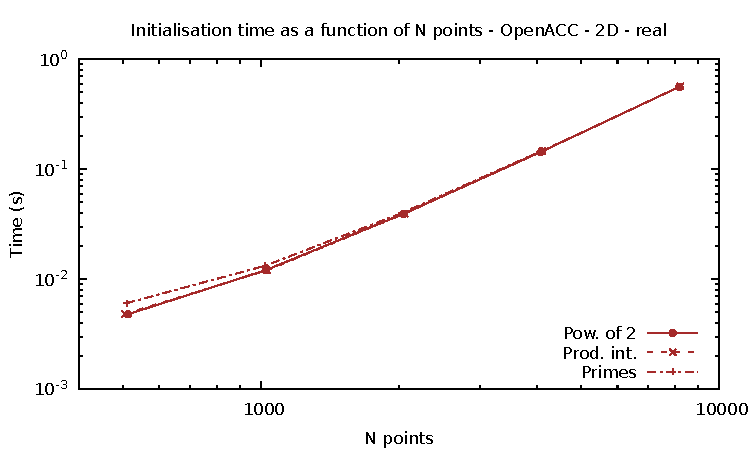
\includegraphics[width=.9\linewidth]{graphs/fft-openacc-2d-pow2-r-init.pdf}
\caption{Intialisation (real)}
\label{FFTACC1DRI}
\end{subfigure}%
\begin{subfigure}{.5\textwidth}
\centering
\includegraphics[width=.9\linewidth]{graphs/fft-openacc-2d-pow2-r-exec.pdf}
\caption{Execution (real)}
\label{FFTACC1DRE}
\end{subfigure}\\
\begin{subfigure}{.5\textwidth}
\centering
%\includegraphics[width=.9\linewidth]{}
\caption{Intialisation (complex)}
\label{FFTACC1DCI}
\end{subfigure}%
\begin{subfigure}{.5\textwidth}
\centering
\includegraphics[width=.9\linewidth]{graphs/fft-openacc-2d-pow2c-exec.pdf}
\caption{Execution (complex)}
\label{FFTACC1DCE}
\end{subfigure}
\caption{Initialisation and execution times as a function of the number of points\\(1 dimension)}
\label{FFTCL1D}
\end{figure}

\begin{figure}[H]
\captionsetup{width=0.8\linewidth}
\centering
\begin{subfigure}{.5\textwidth}
\centering
\includegraphics[width=.9\linewidth]{graphs/fft-2d-pow2-r-init.pdf}
\caption{Intialisation (real)}
\label{FFTPOW21DRI}
\end{subfigure}%
\begin{subfigure}{.5\textwidth}
\centering
\includegraphics[width=.9\linewidth]{graphs/fft-2d-pow2-r-exec.pdf}
\caption{Execution (real)}
\label{FFTPOW21DRE}
\end{subfigure}\\
\begin{subfigure}{.5\textwidth}
\centering
\includegraphics[width=.9\linewidth]{graphs/fft-2d-pow2-c-init.pdf}
\caption{Intialisation (complex)}
\label{FFTPOW21DCI}
\end{subfigure}%
\begin{subfigure}{.5\textwidth}
\centering
\includegraphics[width=.9\linewidth]{graphs/fft-2d-pow2-c-exec.pdf}
\caption{Execution (complex)}
\label{FFTPOW21DCE}
\end{subfigure}
\caption{Initialisation and execution times as a function of the number of points\\(1 dimension)}
\label{FFTPOW21D}
\end{figure}

\begin{figure}[H]
\captionsetup{width=0.8\linewidth}
\centering
\begin{subfigure}{.5\textwidth}
\centering
\includegraphics[width=.9\linewidth]{graphs/fft-2d-r-init.pdf}}
\caption{Intialisation (real)}
\label{FFT1DRI}
\end{subfigure}%
\begin{subfigure}{.5\textwidth}
\centering
\includegraphics[width=.9\linewidth]{graphs/fft-2d-r-exec.pdf}
\caption{Execution (real)}
\label{FFT1DRE}
\end{subfigure}\\
\begin{subfigure}{.5\textwidth}
\centering
\includegraphics[width=.9\linewidth]{graphs/fft-2d-c-init.pdf}
\caption{Intialisation (complex)}
\label{FFT1DCI}
\end{subfigure}%
\begin{subfigure}{.5\textwidth}
\centering
\includegraphics[width=.9\linewidth]{graphs/fft-2d-c-exec.pdf}
\caption{Execution (complex)}
\label{FFT1DCE}
\end{subfigure}
\caption{Initialisation and execution times as a function of the number of points\\(1 dimension)}
\label{FFT1D}
\end{figure}



















\subsubsection{OpenCL}
\includegraphics[height=8cm]{graphs/fft-opencl-3d-pow2-r-init.pdf}\\
\includegraphics[height=8cm]{graphs/fft-opencl-3d-pow2-r-exec.pdf}\\
\includegraphics[height=8cm]{graphs/fft-opencl-3d-pow2-c-init.pdf}\\
\includegraphics[height=8cm]{graphs/fft-opencl-3d-pow2c-exec.pdf}\\
\subsubsection{OpenACC}
\includegraphics[height=8cm]{graphs/fft-openacc-3d-pow2-r-init.pdf}\\
\includegraphics[height=8cm]{graphs/fft-openacc-3d-pow2-r-exec.pdf}\\
\includegraphics[height=8cm]{fft-openacc-3d-pow2c-exec.pdf}\\
\subsubsection{All - powers of 2}
\includegraphics[height=8cm]{graphs/fft-3d-pow2-r-init.pdf}\\
\includegraphics[height=8cm]{graphs/fft-3d-pow2-r-exec.pdf}\\
\includegraphics[height=8cm]{graphs/fft-3d-pow2-c-init.pdf}\\
\includegraphics[height=8cm]{graphs/fft-3d-pow2-c-exec.pdf}\\
\subsubsection{All}
\includegraphics[height=8cm]{graphs/fft-3d-r-init.pdf}\\
\includegraphics[height=8cm]{graphs/fft-3d-r-exec.pdf}\\
\includegraphics[height=8cm]{graphs/fft-3d-c-init.pdf}\\
\includegraphics[height=8cm]{graphs/fft-3d-c-exec.pdf}\\
\subsection{Flatness}
\includegraphics[height=8cm]{graphs/flatness-r-init.pdf}\\
\subsection{CCPPETMR}
\includegraphics[height=8cm]{graphs/fft-ccppetmr-init.pdf}\\
\includegraphics[height=8cm]{graphs/fft-ccppetmr-exec.pdf}\\
\section{Product}
\includegraphics[height=8cm]{graphs/product-r.pdf}\\
\includegraphics[height=8cm]{graphs/product-c.pdf}\\

%\subsectection{Flatness}

%These experiments were carried out with domains whose dimensions were the same #in all directions, that is, squares or cubes. We have observed that there is no clear trend in the way the flatness of the domain affects the performance. Fig. \ref{FLATNESS} shows the performance obtained, in 3 dimensions, for a cuboid containing $512^3$ points whose sides in the $y$ and $z$ directions have identical lengths. We hade defined the flatness as the ratio between the number of points in the $y$ and $x$ directions ($N_y/N_x,\ N_y=N_z$). We varied the proportions of the volume from $512:512:512$ till $2^{24}:2:2$.  \\

%\begin{figure}[H]
%\captionsetup{width=0.8\linewidth}
%\centering
%\begin{subfigure}{.5\textwidth}
%\centering
%\includegraphics[width=.9\linewidth]{graphs/performance/3d-flatness-pow2-r.pdf}
%\caption{Real}
%\label{FLATNESSR}
%\end{subfigure}%
%\begin{subfigure}{.5\textwidth}
%\centering
%\includegraphics[width=.9\linewidth]{graphs/performance/3d-flatness-pow2-c.pdf}
%\caption{Complex}
%\label{FLATNESSC}
%\end{subfigure}
%\caption{Execution time as a function of the flatness of the domain ($N_y/N_x$), for $N_y=N_z$ (3 dimensions, powers of 2, 1 thread)}
%\label{FLATNESS}
%\end{figure}


%\section{Requirements from the CCP}
%We have also benchmarked the FFT libraries in a situation corresponding to a problem encountered by the CCP/PET-MR collaboration, by computing the transform of a series of 32 square complex images whose side consists of 256 points as well as the closest prime number (257) and product of powers of small integers ($2^23^27=252$). As in the other cases, the MKL library performs better than FFTW. None of the other libraries we have considered could be used in this situation. GSL works only in one dimension. The FORTRAN version of FFTPACK does not share that limitation. However all the C/C++ wrappers we have found offer only one-dimensional transforms. Finally FFTPACK is distributed with a licence that is less constraining than the GPL but, nevertheless, the C++ wrapper provided by CASA that we have used is distributed under the GPL v2.

%\begin{figure}[H]
%\captionsetup{width=0.6\textwidth}
%\centering
%\includegraphics[height=8cm]{graphs/ccp/ccp.pdf}
%\caption{Execution time for the transform of 32 complex square images as a function of square side\\(2 dimensions, complex, 1 thread)}
%\label{method}
%\end{figure}

%\section{Acknowledgements}
%This work was funded by under grant .
\begin{thebibliography}{9}

\bibitem{cuda}
\hyperlink{https://developer.nvidia.com/cuda-zone}{https://developer.nvidia.com/cuda-zone}

\bibitem{opencl}
\hyperlink{https://www.khronos.org/opencl/}{https://www.khronos.org/opencl/}
  
\bibitem{fftpack}
\hyperlink{https://www.khronos.org/opencl/}{https://www.khronos.org/opencl/}

\bibitem{openacc}
\hyperlink{https://www.openmp.org/}{https://www.openmp.org/}
  
\bibitem{openmp}
\hyperlink{https://www.openmp.org/}{https://www.openmp.org/}

\bibitem{kokkos}
\hyperlink{https://github.com/kokkos}{https://github.com/kokkos}

\bibitem{cufft}
\hyperlink{https://docs.nvidia.com/cuda/cufft/index.html}{https://docs.nvidia.com/cuda/cufft/index.html}

\bibitem{clfft}
  \hyperlink{https://github.com/clMathLibraries/clFFT}{https://github.com/clMathLibraries/clFFT}
  
\bibitem{accfft}
\hyperlink{http://accfft.org/}{http://accfft.org/}

\bibitem{casa}
McMullin, J. P., Waters, B., Schiebel, D., Young, W., Golap, K.,
{\it Astronomical Data Analysis Software and Systems XVI},
ASP Conf. Ser. 376, ed. R. A. Shaw, F. Hill, D. J. Bell (San Francisco, CA: ASP), 127

\bibitem{code}
\hyperlink{git@github.com:SoftwareOutlook/GPU.git}{git@github.com:SoftwareOutlook/GPU.git}
    
\bibitem{ccppetmr}
\hyperlink{https://www.ccppetmr.ac.uk/}{https://www.ccppetmr.ac.uk/}

\bibitem{softwareoutlook}
\hyperlink{https://www.softwareoutlook.ac.uk/}{https://www.softwareoutlook.ac.uk/}
  
\end{thebibliography}

\end{document}
